\section{Some theory}

\subsection{Bayesian filtering}
\label{bayesian_filtering}

\subsubsection{Chapman - Kolmogorov prediction}

\begin{equation}
    p(x_k \vert z_{1:k-1}) = \int p(x_k \vert x_{k-1}) \: p(x_{k-1} \vert z_{1:k-1}) \: dx_{k-1}
\end{equation}

Assuming a Gaussian and linear transition model alongside a Gaussian prior.

\begin{align}
p(x_k \vert x_{k-1}) &\sim \mathcal{N}(x_k; F x_{k-1}, Q) \\
p(x_{k-1} \vert z_{1:k-1}) &\sim \mathcal{N}(x_{k-1}; \hat{x}_{k-1}, \hat{P}_{k-1})
\end{align}

Then it can be shown that

\begin{equation}
    \int \mathcal{N}(x_k; F x_{k-1}, Q) \: \mathcal{N}(x_{k-1}; \hat{x}_{k-1}, \hat{P}_{k-1}) \: dx_{k-1} = \mathcal{N}(x_k; \hat{x}_{k \vert k-1}, \hat{P}_{k \vert k-1})
\end{equation}
\begin{align}
    \hat{x}_{k \vert k-1} &= F \hat{x}_{k-1} \\
    \hat{P}_{k \vert k-1} &= F \hat{P}_{k-1} F^T + Q
\end{align}

\subsubsection{Bayes update}
Because of the proportionality in the following equation (TODO: explain why the proportionality must hold), we do not need to find the value in the denominator. The pdf can just be normalized such that it integrates to one.

\begin{equation}
    p(x_k \vert z_{1:k}) = \frac{p(z_k \vert x_k) p(x_k \vert z_{1:k-1})}{p(z_k \vert z_{1:k-1})} \propto p(z_k \vert x_k) p(x_k \vert z_{1:k-1})
\end{equation}

\subsubsection{Predicted likelihood}

As mentioned above, the value of the so-called predicted likelihood is not always necessary, but in Multi object tracking it may nonetheless be very useful. This is because this density tells us something about how likely a given measurement is, given it comes from the object we are tracking. This value is therefore very useful for the data association.

\begin{equation}
    p(z_k \vert z_{1:k-1}) = \int p(z_k \vert x_k) p(x_k \vert z_{1:k-1}) dx_k
\end{equation}

\subsection{Modeling clutter}
Clutter are detections that originate from sources that is not a target we want to track. Clutter is assumed to be random and originate from noise in the detector. Consider a sensor with a field of view in $R^n$ of volume $V$. Let $\lambda$ denote the expected number of clutter detections per unit volume. It is then clear that the expected number of clutter measurements in the sensors FOV is $ \mathbb{E}[\vert C_k \vert] = \lambda V $. 
\medskip

By discretizing the sensor and letting the resolution tend to infinity, we can argue that $\vert C_k \vert$ is Poisson distributed and that $C_k$ is a Poisson point process (PPP). 

\begin{definition}{Poisson point process clutter model}
\textbf{Clutter} $C_k$ is a random set / random matrix of a random number of random vectors. $C_k$ is defined such that:
\begin{itemize}
    \item $C_k = [c^1_k, c^2_k, \ldots , c^{m_k}_k]$
    \item $m_k \sim \text{Po}(\lambda V) $
    \item Given $m_k$, the vectors $c^1_k, c^2_k, \ldots , c^{m_k}_k$ are i.i.d. where $c_k^j \sim \text{Uniform}(V)$ and $V$ is the sensor FOV.
    \item The PPP can be parameterized by a spatial intensity function $\lambda(x) \geq 0$, where the rate is $\bar{\lambda} = \int \lambda(x) \: dx$
    \item A spatial pdf can be obtained as $f_c(x) = \frac{\lambda(x)}{\bar{\lambda}}$
    \item The pdf of the PPP is then 
    \[
    p(C_k) = p(C_k, m_k) = p(m_k) \, p(C_k \vert m_k) = \text{Po}(m_k; \bar{\lambda}) \prod_{i=1}^{m_k} f_c(c^i_k) = \frac{\exp(-\bar{\lambda})}{m_k!} \prod_{i=1}^{m_k} \lambda(c_k^i)
    \]
\end{itemize}
\end{definition}

\subsection{Modeling misdetections}
Objects we are trying to detect may or may not be detected at each timestep. In the single target case, we assume that a target is always present and that the target is detected with a probability $P^D(x_k)$. $O_k$ is a variable that contains the possibility that the target is either not detected or detected and generates a measurement from the measurement model $h(o_k \vert x_k)$. This can be summed up in the following way.

\begin{definition}{Misdetection model}
Given $x_k$, the det of vectors in $O_k$ is a Bernoulli random finite set distributed according to:
\begin{equation}
    p(O_k \vert x_k) = 
    \begin{cases}
        1 - P^D(x_k) & \text{if } O_k = [] \\
        P^D(x_k) \: h(o_k \vert x_k) & \text{if } O_k = o_k
    \end{cases}
\end{equation}
\end{definition}

We will later see that we need $P^D(x_k)$ to be constant in order to simplify the filtering greatly.

\subsection{Measurement model}
With the clutter model and detection model at hand we can define the measurement model for single target tracking. 

\begin{definition}{Measurement model}
Given $O_k$ and $C_k$ defined as above, the measurement $Z_k$ is defined as:
\begin{equation}
    Z_k = \Pi(O_k, C_k)
\end{equation}
where $\Pi$ is an operator that combines and randomly shuffles the columns of a matrix.
\end{definition}

The definition above simply means that the measurement $Z_k$ contains a random number of clutter vectors and possibly a target measurement, but we do not know which is which. We will soon introduce association hypotheses, meaning theories about which column of $Z_k$ that corresponds to the target. 

\begin{definition}{Association hypothesis}
The association hypotheses are denoted by $\theta$ and defined as:
\begin{equation}
    \theta = 
    \begin{cases}
        i > 0 & \text{if $z^i$ is an object detection} \\
        0 & \text{if the object is undetected}
    \end{cases}
\end{equation}
\end{definition}

For filtering we seek to obtain the equation for $p(Z \vert x)$, omitting the time for readability. The following will just be an outline of the derivation, leaving out most of the algebra.

\begin{equation*}
    p(Z \vert x) = p(Z, m \vert x) = \sum_{\theta = 0}^{m} p(Z, m, \theta \vert x) = \sum_{\theta = 0}^{m} p(Z \vert m, \theta, x) \: p(\theta, m \vert x)
\end{equation*}
\begin{equation}
    = \left[ (1 - P^D(x)) + P^D(x) \: \sum_{\theta = 1}^{m} \frac{h(z^\theta \vert x)}{\lambda(z^\theta)} \right] \: \frac{exp(-\bar{\lambda})}{m!} \prod_{i = 1}^{m} \lambda(z^i)
\end{equation}

\subsection{Single target tracking}
From \ref{bayesian_filtering} we know that the posterior is given by the following equation. Notice that the proportionality has swallowed some terms not dependent on $x$.
\begin{equation}
    \label{eq:mes_mod}
    p(x \vert Z) \propto p(x) \: p(Z \vert x) \propto p(x) \: \left[ (1 - P^D(x)) + P^D(x) \: \sum_{\theta = 1}^{m} \frac{h(z^\theta \vert x)}{\lambda(z^\theta)} \right]
\end{equation}
It can also be shown that the joint distribution of $x$ and $\theta$ given $Z$, can be written as a constant times a pdf over $x$.
\begin{equation*}
    p(x, \theta \vert Z) = w_\theta p_\theta(x)
\end{equation*}
The following three relations then follow trivially.
\begin{equation*}
    w_\theta = Pr(\theta \vert Z)
\end{equation*}
\begin{equation*}
    p_\theta(x) = \frac{p(x, \theta \vert Z)}{w_\theta} = \frac{p(x, \theta \vert Z)}{Pr(\theta \vert Z)} = p(x \vert \theta, Z)
\end{equation*}
\begin{equation}
    \label{eq:also_mes_mod}
    p(x \vert Z) = \sum_{\theta = 0}^{m} w_\theta \: p_\theta(x)
\end{equation}

With the knowledge from \autoref{eq:also_mes_mod}, we now want to rewrite \autoref{eq:mes_mod} into that form. This may seem like a complication, but we will later see that the equations simplify nicely with a few assumptions. The transformation is nothing more than taking each term, integrating it and then multiply and divide each component by that integral. Thus, so far changing nothing.

We get $p(x|Z) = \sum_{\theta=0}^{m} w_\theta p_\theta(x)$, where

\[
\theta = 0: \quad \text{Object is undetected} \quad
\begin{cases}
\tilde{w}_0 = \int p(x)(1 - P^{\mathrm{D}}(x)) \, \mathrm{d}x \\[2mm]
p_0(x) = \dfrac{p(x)(1 - P^{\mathrm{D}}(x))}{\int p(x')(1 - P^{\mathrm{D}}(x')) \, \mathrm{d}x'},
\end{cases}
\]

\[
\theta \in \{1, 2, \ldots, m\}: \quad z^\theta \text{ is object detection} \quad
\begin{cases}
\tilde{w}_\theta = \dfrac{1}{\lambda(z^\theta)} \int p(x) P^{\mathrm{D}}(x) g(z^\theta \vert x) \, \mathrm{d}x \\[2mm]
p_\theta(x) = \dfrac{p(x) P^{\mathrm{D}}(x) g(z^\theta \vert x)}{\int p(x') P^{\mathrm{D}}(x') g(z^\theta \vert x') \, \mathrm{d}x'},
\end{cases}
\]

and $w_\theta \propto \tilde{w}_\theta$.

\textbf{Assuming constant detection probability} \\
Immediate simplifications can be done by assuming $P^D(x) = P^D$. Whether this assumption is valid or not is highly dependent on the detector giving out measurements, and possibly environmental considerations, but in many cases this is fair to assume. In cases where this assumption is not valid or good enough, other pdf approximations such as particle filtering must be used for this algorithm to be usable. Using $P^D$, the posterior simplifies to:

\[
\theta = 0: \quad \text{Object is undetected} \quad
\begin{cases}
\tilde{w}_0 = 1 - P^D \\[2mm]
p_0(x) = p(x)
\end{cases}
\]

\[
\theta \in \{1, 2, \ldots, m\}: \quad z^\theta \text{ is object detection} \quad
\begin{cases}
\tilde{w}_\theta = \dfrac{P^D}{\lambda(z^\theta)} \int p(x) g(z^\theta \vert x) \, \mathrm{d}x \\[2mm]
p_\theta(x) = \dfrac{p(x) g(z^\theta \vert x)}{\int p(x') g(z^\theta \vert x') \, \mathrm{d}x'},
\end{cases}
\]

Looking at $p_\theta(x)$, we see that it is a non-negative integrable function that integrates to one. This means $p_\theta(x)$ is a pdf, and thus we can temporarily ignore the normalization constant since $p_\theta(x)$ only carries information about the shape of the pdf while the weight is captured in $\tilde{w}_\theta$.

\textbf{Gaussian linear assumptions} \\
The following standard filtering assumptions will now be applied.
\begin{align*}
    p(x) &= \mathcal{N}(x; \mu, P) \\
    h(z \vert x) &= \mathcal{N}(z; Hx, R)
\end{align*}

Under these assumptions, we see that the solution must be the standard Kalman filter update equations presented in \autoref{bayesian_filtering}. The final solution can then be written as:

\[
p(x \vert Z) = \sum_{\theta=0}^{m} w_\theta \, p_\theta(x), \qquad
w_\theta = \dfrac{\tilde{w}_\theta}{\displaystyle\sum_{\theta'=0}^{m} \tilde{w}_{\theta'}}.
\]

\[
\theta = 0: \quad \text{Object is undetected} \quad
\begin{cases}
\tilde{w}_0 = 1 - P^D \\[2mm]
p_0(x) = \mathcal{N}(x; \mu, P)
\end{cases}
\]

\[
\theta \in \{1, 2, \ldots, m\}: \quad z^\theta \text{ is object detection} \quad
\begin{cases}
\tilde{w}_\theta = \dfrac{P^D}{\lambda(z^\theta)} \, \mathcal{N}(z^\theta; H\mu, S) \\[2mm]
p_\theta(x) = \mathcal{N}(x; \mu_\theta, P_\theta)
\end{cases}
\]

Where the innovation covariance, Kalman gain, and updated moments are given by
\begin{align*}
    S &= HPH^\top + R \\
    K &= PH^\top S^{-1} \\
    \mu_\theta &= \mu + K\left(z^\theta - H\mu\right) \\
    P_\theta &= P - KHP.
\end{align*}

Notice that this is the stage where the weights are finally normalized, giving an actual pdf. This solution is a Gaussian mixture of all the different hypotheses, weighed by how likely the measurements are according to the model. This solution could in theory be implemented as is, but only for a very short time. When the algorithm is iterated across multiple rounds of measurements, there will be introduced $m$ times as many hypotheses at each timestep. This will therefore get out of hand very quickly and further approximations to keep the number of hypotheses from blowing up must therefore be introduced.

\subsubsection{Nearest neighbor algorithms}
One way to approach hypotheses reduction is to only keep the most probable hypothesis after each iteration. This is essentially a MAP approach to the tracking problem. Each iteration you get rid of all, but the hypothesis with the highest weight, and then use that hypothesis as prior in the next iteration. One possible problem with this approach is that it often underestimates the variance of the true distribution, which can lead to it getting stuck believing the wrong thing for a couple of iterations (SOURCE?).

\subsubsection{Probabilistic data association filtering (PDAF)}
One other approach is to merge all hypotheses into a single Gaussian after each iteration. 

\begin{definition}{Gaussian mixture reduction}
Given a Gaussian mixture $p(x) = \sum_{\theta=0}^{m} w_\theta \, \mathcal{N}(x; \mu_\theta, P_\theta)$ with $\sum_{\theta=0}^{m} w_\theta = 1$, the mixture can be reduced to a single Gaussian $\mathcal{N}(x; \bar{\mu}, \bar{P})$ with identical first and second moments, given by

\[
\bar{\mu} = \sum_{\theta=0}^{m} w_\theta \, \mu_\theta
\]

\[
\bar{P} = \sum_{\theta=0}^{m} w_\theta P_\theta + w_\theta (\mu_\theta - \bar{\mu})(\mu_\theta - \bar{\mu})^T
\]
\end{definition}

It can be shown that this approach is the Gaussian pdf that minimizes the Kullback-Leibler (KL) divergence, and thus it is the Gaussian most "similar" to the mixture.

\subsubsection{Gaussian sum filtering}
Gaussian sum filtering is a collective term of methods where more than one hypothesis is kept after each estimation cycle. In general, you define a maximum number of hypotheses you want to be left with after each estimation cycle. You can then either pick the $N$ most likely hypotheses and let the next prior be a mixture of these, or you can merge similar hypotheses before picking the $N$ most likely. If merging is to be done, you will need to effectively search for and merge similar Gaussians. Depending on your scenario this may or may not be needed and many times nearest neighbors or PDAF will be more than necessary.

\subsection{N-vector as a position representation}
When tracking objects on earth over large distances, we require some way of representing global position. One of the most popular representations is latitude/longitude. However, this representation suffers from singularities at the poles and is discontinuous at the Date line. An alternative representation is N-vector \parencite{k_gade_2010}. It is defined as a 3D unit normal vector to the surface of earth and is expressed in an earth fixed coordinate frame $E$. Further descriptions will therefore use $n^E$ to denote n-vectors in coordinate frame $E$. N-vectors does not suffer from discontinuities or singularities, and many problems can be solved by simple vector algebra \parencite{k_gade_2010}. 

\subsection{Tracking using N-vector}
\label{sec:tracking_n_vector}
One of the issues of tracking moving vessels over large geographical areas is error introduced by the curvature of the earth. One might think that such errors are way too small to be worth compensating for, but consider a case with a fast moving vessel and infrequent measurements. A satellite based measurement might only arrive every 1.5 hours and a fast moving vessel can cover 50 to 80 kilometers during that time. DEFINE THE AMOUNT OF ERROR. A tempting approach is therefore to do the Chapman - Kolmogorov prediction along the earths' curvature, and only use flat earth approximations for the local Bayes update. The following description of a prediction and Kalman update using N-vector formulation is outlined in \parencite{b_gade_2024}, so this is merely a presentation of that work. I will now present a single step of the estimation cycle using a single measurement. It is worth noting that there is a sign convention difference between the algorithm presented in \parencite{b_gade_2024} and what will be presented here. This is due to the way the error state is defined, but it makes no difference in the actual implementation.
\medskip

\textbf{Step 0: The prior} \\
From the last estimation cycle we have predicted position $n^E_{k \vert k-1}$ as an N-vector. A measurement $n^E_{k, meas}$ is received. The measurement is expressed in the same global N-vector frame as the predicted position.

\textbf{Step 1: The innovation} \\
The measurement and predicted position is assumed close enough so that their difference can be expressed in the local East - North frame centered around the predicted position $n^E_{k \vert k-1}$. This can trivially be achieved by following the steps in Example 1 at \parencite{ffi_nvector}. We denote this local East - North innovation by $\epsilon^N_k$

\textbf{Step 2: Local Kalman update} \\
Using the 2D innovation $\epsilon^N_k$ we can do a standard Kalman filter update calculation. The resulting states, $\widehat{\delta p}_{k \vert k-1}$ and $\widehat{\delta v}_{k \vert k-1}$, can be thought of as the estimated error in position and velocity. For completeness the equations will be stated explicitly. 

\begin{align}
S_k &= H P_{k|k-1} H^T + R^N_k, \\[4pt]
K_k &= P_{k|k-1} H^T S_k^{-1}, \\[4pt]
\begin{bmatrix}
\widehat{\delta p}_{k|k-1} \\
\widehat{\delta v}_{k|k-1}
\end{bmatrix}
&= K_k\, \epsilon^N_k, \\[4pt]
P_{k|k} &= (I - K_k H)\, P_{k|k-1}.
\end{align}

Two things worth noting; for a positional measurement, as we have in this example, we simply use $H = [I \: 0]$. Also, the measurement covariance matrix $R^N_k$ should be defined in the local East - North frame, the same as $\epsilon^N_k$.

\textbf{Step 3: injection} \\
Using the error estimates $\widehat{\delta p}_{k \vert k-1}$ and $\widehat{\delta v}_{k \vert k-1}$, we can now update the predicted states $n^E_{k \vert k-1}$ and $v^N_{k \vert k-1}$. Injection of the velocity is straightforward while the corrected position is obtained by following Example 2 in \parencite{ffi_nvector}. This operation is denoted by the function $g$.

\begin{align}
    v^N_{k \vert k} &= v^N_{k \vert k-1} + \widehat{\delta v}_{k \vert k-1} \\
    n^E_{k \vert k} &= g(n^E_{k \vert k-1}, \widehat{\delta p}_{k \vert k-1})
\end{align}

\textbf{Step 4: Great circle prediction} \\
Prediction is done using a constant velocity model along the curvature of the earth. The predicted N-vector is given by \autoref{eq:great_circle_prediction} while the velocity is unchanged. However, we still need to reexpress the velocity in the local East - North frame of the new predicted point $n^E_{k+1 \vert k}$.

\begin{equation}
    n^{E}_{k+1|k} = n^{E}_{k|k} \cdot \cos \left( \frac{\lvert v_{k|k}\rvert \cdot \Delta t}{r} \right)
 +
\operatorname{unit}\!\left(v^{E}_{k|k}\right) \cdot \sin\left( \frac{\lvert v_{k|k}\rvert \cdot \Delta t}{r} \right)
\label{eq:great_circle_prediction}
\end{equation}
\begin{equation*}
    v^N_{k+1 \vert k} = v^N_{k \vert k} \: (\text{re-expressed in the new N-frame, centered at } n^E_{k+1 \vert k})
\end{equation*}

Note that $\lvert v_{k|k}\rvert$ is independent of frame. This is because the length of the vector, the absolute velocity, is independent of frame. $r$ is the mean radius of the Earth.
\medskip

The covariance $P_{k+1 \vert k}$ is also predicted. This is done by the standard Kalman filter prediction with the standard constant velocity matrix $F$.

\begin{equation}
    P_{k+1 \vert k} = F P_{k \vert k} F^T + Q^N , \quad 
    F = \begin{bmatrix}
        I & \Delta t I \\
        0 & I 
    \end{bmatrix}
\end{equation}

The convoluted position prediction alongside the simple covariance prediction might look dubious at first glance, but the underlying constant velocity model is the same. It is just mapped to the great circle approximation of the earth in the position. The covariance is still defined in the 2D plane locally.

\textbf{Step 5: Repeat} \\
Use the predicted position and velocity, $n^{E}_{k+1|k}$ and $v^N_{k+1 \vert k}$, as inputs to the next estimation cycle when a new measurement is received.

\subsection{Gating using N-vector}
Gating is important.

\subsection{Clutter on a sphere}
A standard clutter model used for target tracking is the uniform Poisson clutter model. It is parameterized by the clutter intensity $\lambda_c$, which is the expected number of clutter measurements per unit area/volume. Each clutter measurement is independent, and uniformly distributed within the measurement area. In a rectangular measurement area the generation of a clutter measurement is trivial.

\begin{equation*}
    x = \mathcal{U}(\text{min}_x, \text{max}_x) \quad y = \mathcal{U}(\text{min}_y, \text{max}_y)
\end{equation*}

We would now like to sample uniform clutter on the surface of a sphere, the measurement area defined by a maximum angle $\theta_{max}$ between N-vectors of the center and the measurement rim. This is the same approach used earlier for gating. An illustration of the uniform clutter can be seen in \autoref{fig:spherical_cap}.

\begin{figure}[htp]
    \centering
    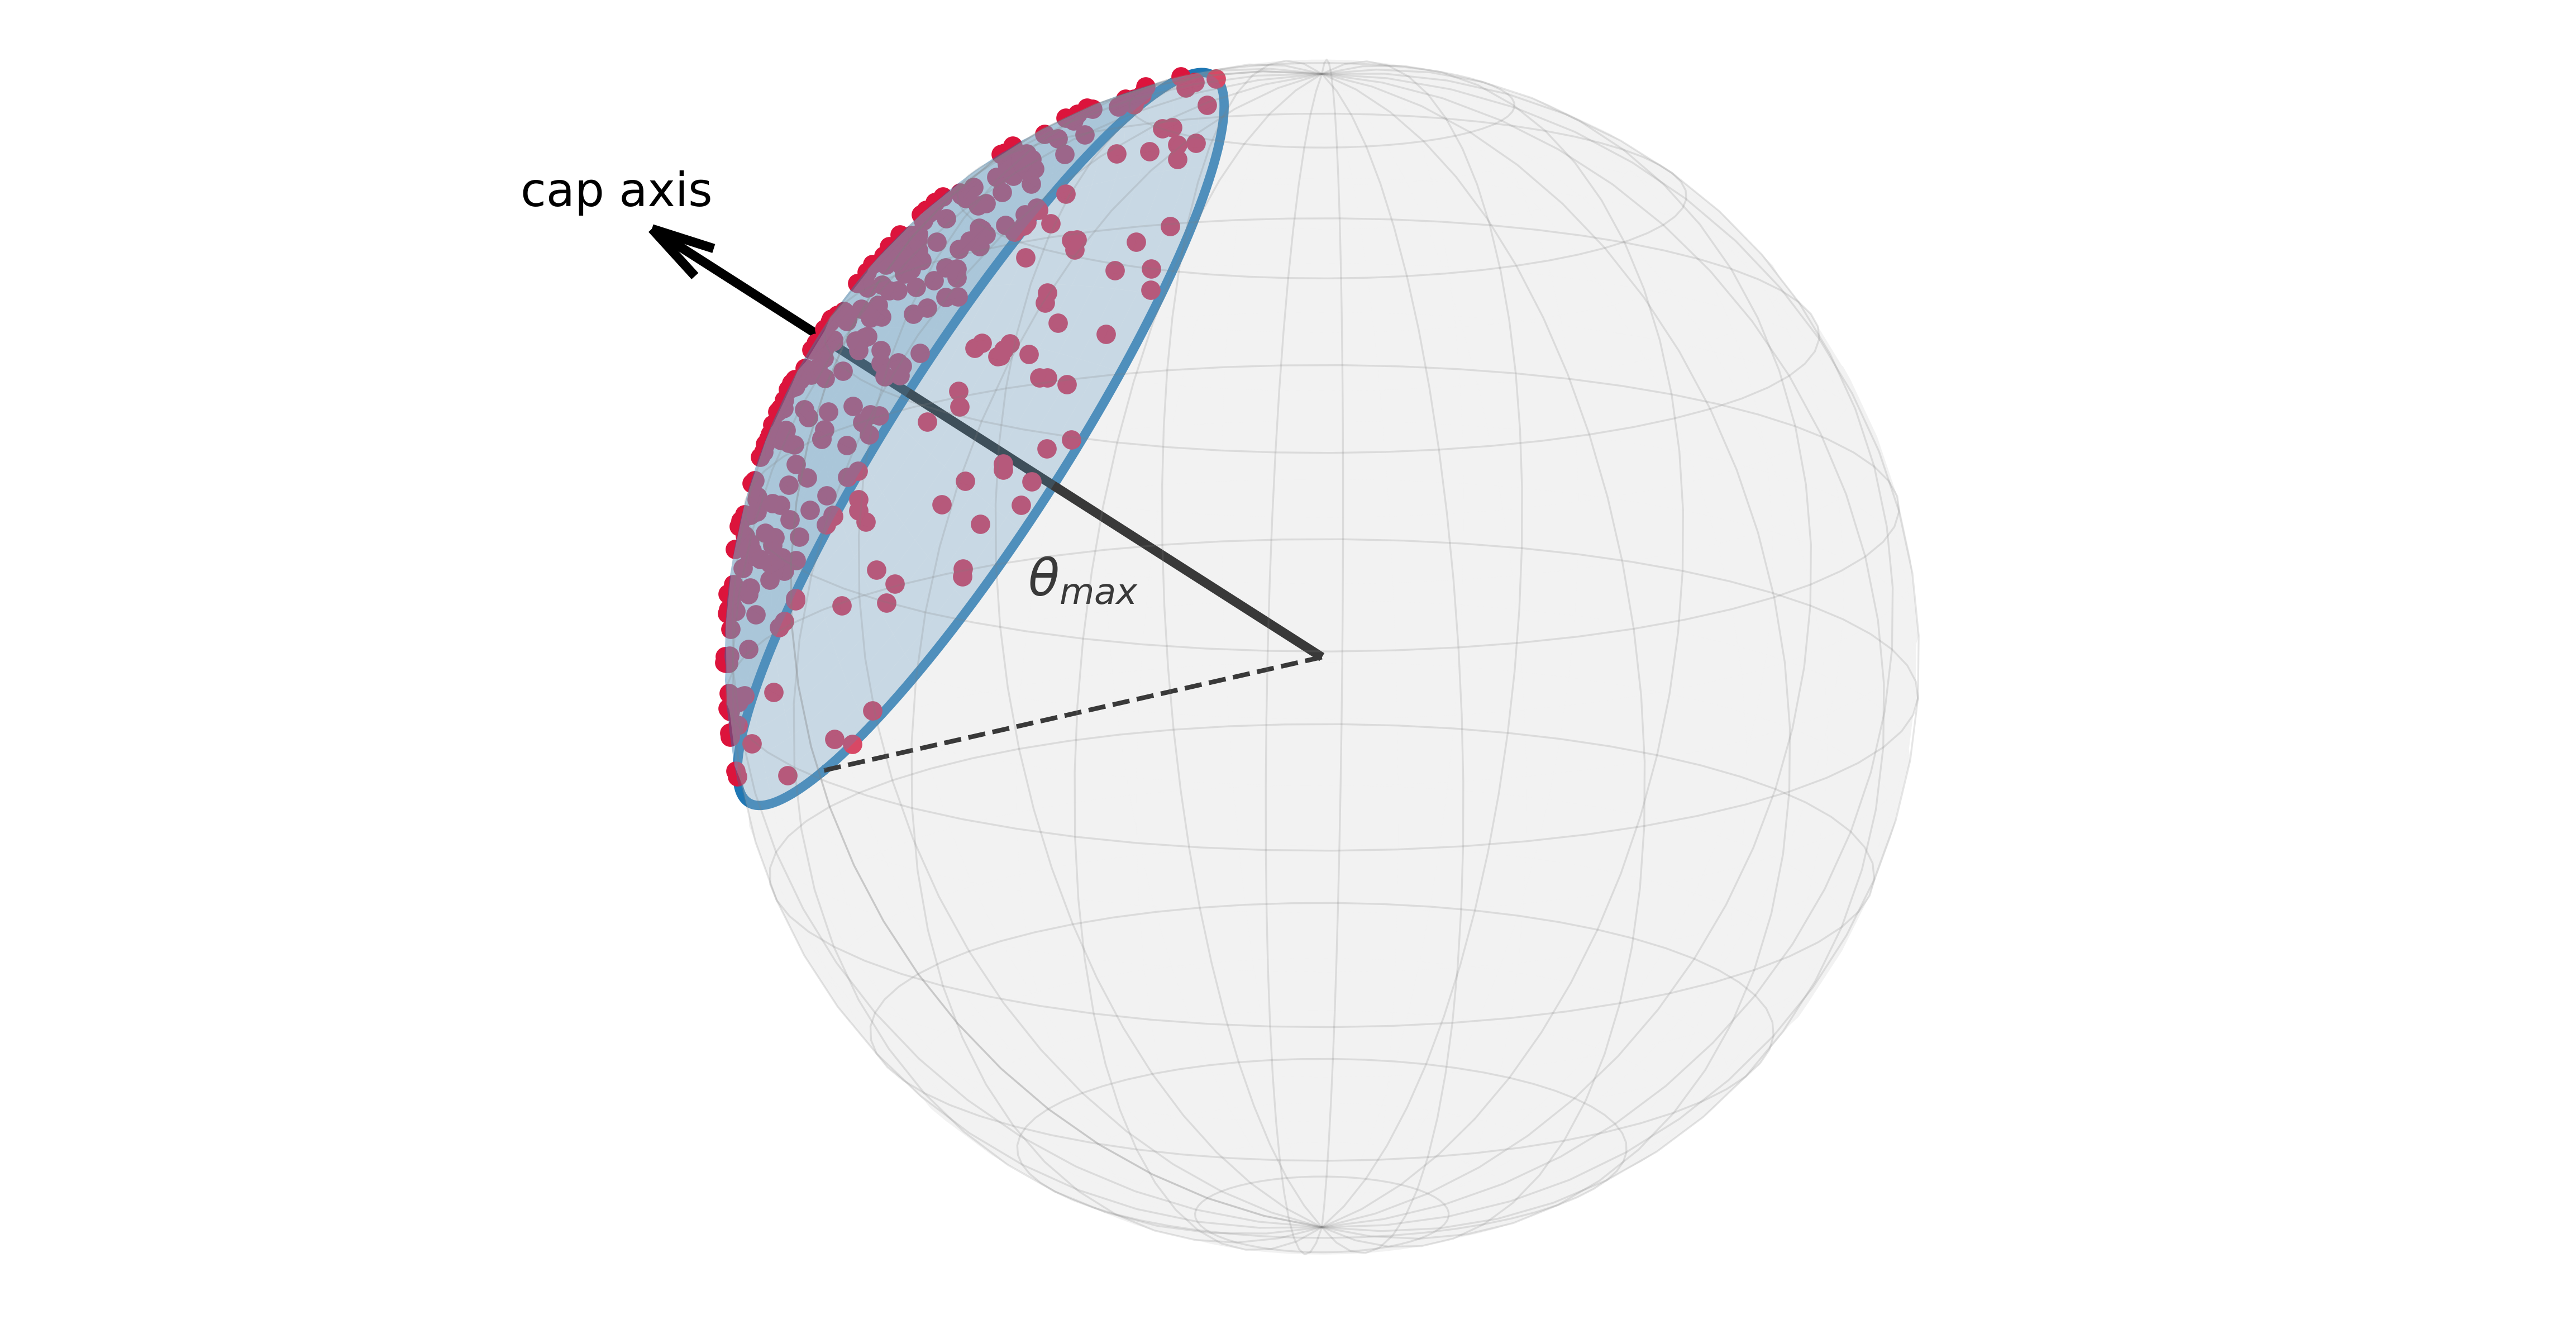
\includegraphics[width=0.8\textwidth]{Images/spherical_cap.png}
    \caption{Points sampled uniformly on a spherical cap, centered around an arbitrary axis.}
    \label{fig:spherical_cap}
\end{figure}

The first part of sampling clutter is to sample the number of clutter measurements, or the cardinality of the Poisson point process if you want. We denote this number $m_k$ and sample it from a Poisson distribution $m_k \sim \text{Po}(\lambda_c A)$. The surface area $A$ of a spherical cap, can be parameterized a few different ways, but using $R$ as the radius of the sphere and $\theta_{max}$ is the most natural in this case. The area is then given by the following formula \parencite{spherical_cap}.

\begin{equation*}
    A = 2 \pi R^2 (1 - \cos(\theta_{max}))
\end{equation*}

The clutter measurements should then be uniformly distributed on the spherical cap. The derivation is explained in detail in \parencite{clutter_sphere}, so I will only touch over the main points here. 
\medskip

We can parameterize the points on the spherical cap by the cap axis (N-vector), radial distance from the cap axis ($\theta \in [0, \theta_{max}]$) and angle between the point and some arbitrary reference point ($\psi \in [0, 2 \pi]$). The angle $\psi$ is illustrated in \autoref{fig:psi_illustration}. We can then sample two independent uniform distributions and get uniform points on the spherical cap by the following transformations.

\begin{figure}[htp]
    \centering
    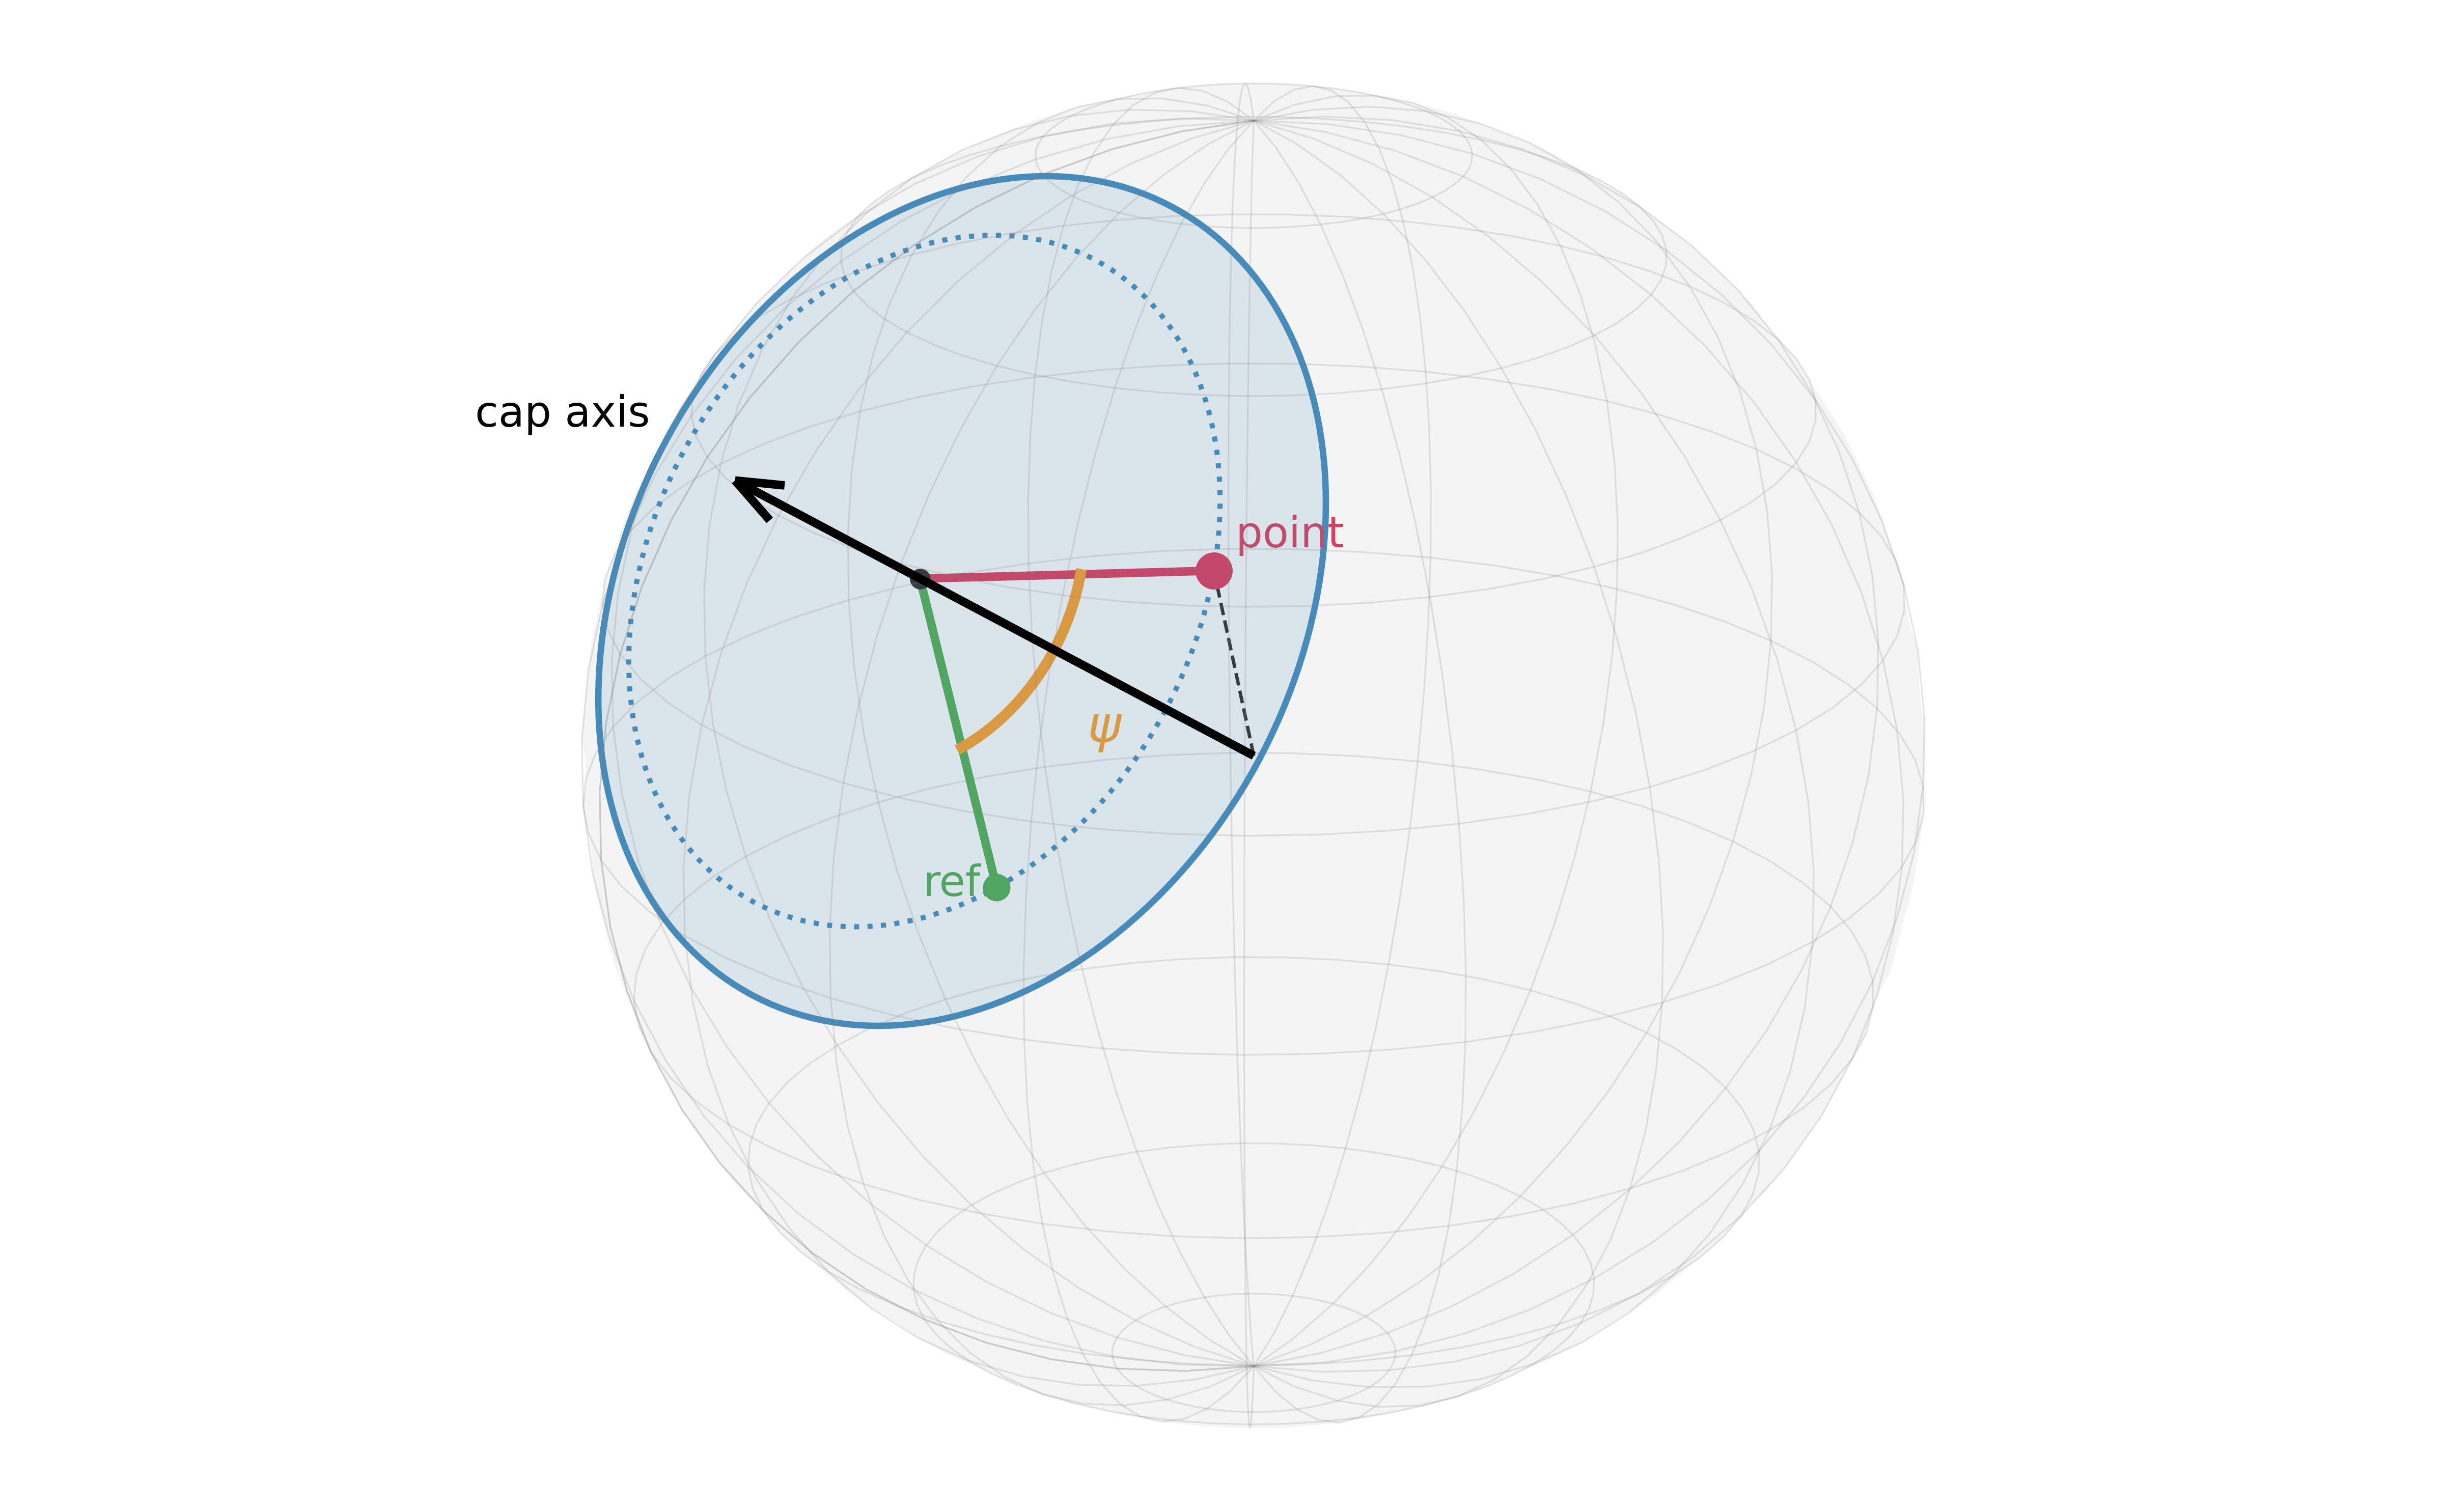
\includegraphics[width=0.8\textwidth]{Images/psi_illustration.png}
    \caption{An illustration of the angle $\psi$}
    \label{fig:psi_illustration}
\end{figure}

\begin{equation*}
    U_1 = \mathcal{U}(0, 1) \quad U_2 = \mathcal{U}(0, 2 \pi)
\end{equation*}

\begin{align*}
    \psi &= U_2 \\
    z &= \cos(\theta_{max}) + U_1 (1-\cos(\theta_{max})) \\
    \theta &= \cos^{-1}(z)
\end{align*}

The uniform point can then be returned as an N-vector by following Example 8 in \parencite{ffi_nvector}. Note that since the points sampled are random and uniform, the result is invariant to rotation about the cap axis. This means that it is not necessary to specify $\psi$ and $\theta$ in the correct East - North frame.